\documentclass[thesis.tex]{subfiles}

\begin{document}
\chapter{Event Reconstruction}
\label{ch3}

Physics objects in CMS are reconstructed using the particle-flow (PF) algorithm~\cite{PARTICLEFLOW}, which identifies each particle through an optimized combination of signals of all sub-detectors.
The PF candidates are classified as photons, charged hadrons, neutral hadrons, electrons, or muons.
Photons are reconstructed by clustering energy deposits in the ECAL. 
Tracks are first formed using hits in the inner tracker and then extrapolated to the calorimeter and muon chambers.
If a track is geometrically close to ECAL and HCAL clusters within a certain distance, they are linked together to form a charged hadron.  
ECAL and HCAL clusters without associated tracks are identified as neutral hadrons. 
Muons are formed if the tracks can be associated with segments in muon stations. 
Electrons are reconstructed by associating tracks to ECAL clusters, and their energies are determined from a combination of the track momentums, calorimeter energy and a sum of all bremsstrahlung photons. 
Fig. \ref{fig:PF} illustrates the response of different types of PF candidates in CMS. 
The algorithms for the reconstruction of different PF elements are detailed in the following sections. 

\begin{figure*}[htb]
	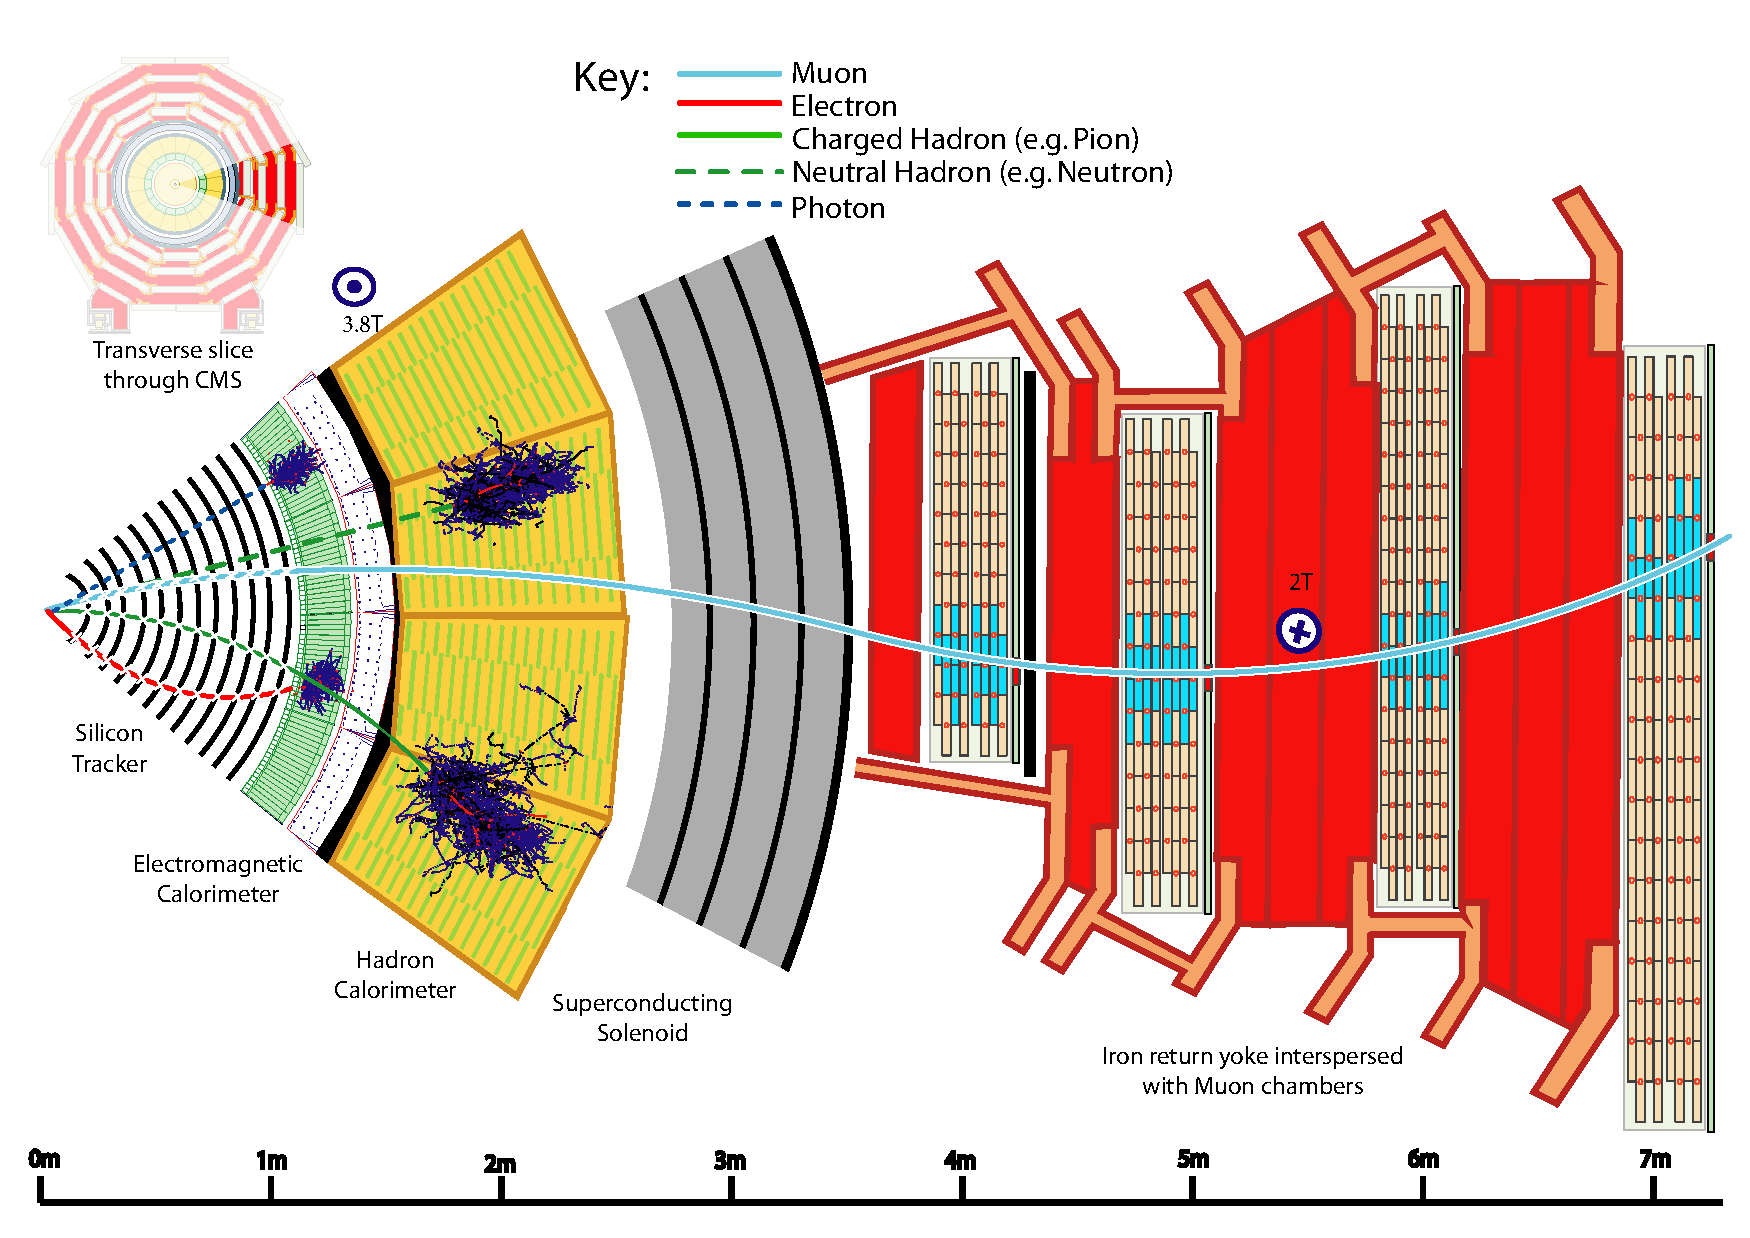
\includegraphics[width=0.9\textwidth]{Fig/ParticleFlow.pdf}
	\caption{A sketch of the responses of different types of particles in a transverse slice of the CMS detector. The muon and the charged pion are positively charged, and the electron is negatively charged. Reprint from ~\cite{PARTICLEFLOW}. }
	\label{fig:PF}
\end{figure*}


\section{Tracks}
The tracker is the subdetector that is closest to the collision point of the LHC. 
An accurate reconstruction of tracks is essential for the identification of charged particles and measurement of momentums. 
The vertexes of the pp collisions can be reconstructed by taking the intersection points of the tracks.
A correct estimation of the positions of interaction vertexes is essential for both object identification and pileup mitigation.
Therefore, the track-finding algorithms must be able to fully exploit the capabilities of the tracker and reconstruct the tracks with high efficiency and accuracy. 

A Combinatorial Track Finder (CTF) based on extended Kalman filter (KF) is used for track reconstruction~\cite{TrackPF}. 
The CTF reconstruction sequence is performed in several iterations, with the initial interactions targeting at easy-identifiable tracks whereas later interactions dealing with more complex situations. 
Hits associated with the tracks in each iteration is removed from later iterations in order to reduce the complexity for reconstructing more difficult tracks. 
The CTF generates track seeds in the inner layers of the tracker and constructs the tracks outwards. 
Each CTF iteration proceeds in four steps:

\begin{itemize}
	\item Seed generation. The track seeds are a set of hits whose patterns are compatible with charged-particle trajectories. 
		In the first few iterations, triplets of pixel hits or mixed pixel pairs with additional vertex constraint are used as seeds. 
		In later iterations, matched hits from the double-layer strip detector are also used to form the seeds. 
	\item Track finding. The seed trajectories are extrapolated outwards and inwards to search for other tracker hits compatible with the expected path of a charged particle. The algorithm is based on Kalman filter method. 
	\item Track fitting. A final fit to the track trajectories is performed to smooth the tracks and provide the best possible estimation of the track parameters. The $\chi^2$ value is saved for each track.
	\item Track selection. Tracks are selected with a list of criteria, including requirements on the minimum number of layers with associated hits, requirements on the maximum number of layers containing no associated hits, upper bounds on $\chi^2$, and thresholds on other track parameters. These selections help remove the fake tracks. 
\end{itemize}

The CTF algorithms reconstruct tracks with high efficiency over the pseudorapidity range of the tracker.
An average reconstruction efficiency of 94\% in the barrel and 85\% in higher $|\eta|$ regions is achieved for charged particles of $p_T >$ 0.9 GeV in $t\bar{t}$ MC events. 

The primary vertex, which is defined as the vertex with the highest $\sum p_T^2$ of associated tracks, is reconstructed by clustering the prompt tracks and performing fits to determine their common vertex. 
Tracks entering the primary vertex finding are required to satisfy cuts on the transverse impact parameter, the number of track hits and the normalized $\chi^2$.
The achieved vertex spatial resolution is 10-12 $\mu m$.

\section{Photons}
\label{sec:reco-photon}

Photons are reconstructed from clusters of energy deposits in the ECAL~\cite{PhotonPF}.
The pulse from each crystal is digitized by a 12 bit ADC running at 40MHz and a set of 10 consecutive samples is recorded for amplitude reconstruction.
In the high luminosity conditions, the pulse contains not only the signals from the current bunch collision but also the contributions from previous pileup bunches.
To mitigate the out of time pileup, a multi-fit algorithm is used to reconstruct the signal amplitudes by estimating the in-time signal amplitude with up to 9 out-of-time amplitudes.
Figure \ref{fig:multifit} shows examples of fitted pulses for simulated events in the EB and the EE with 20 average pileup interactions.

\begin{figure*}[hbt]
	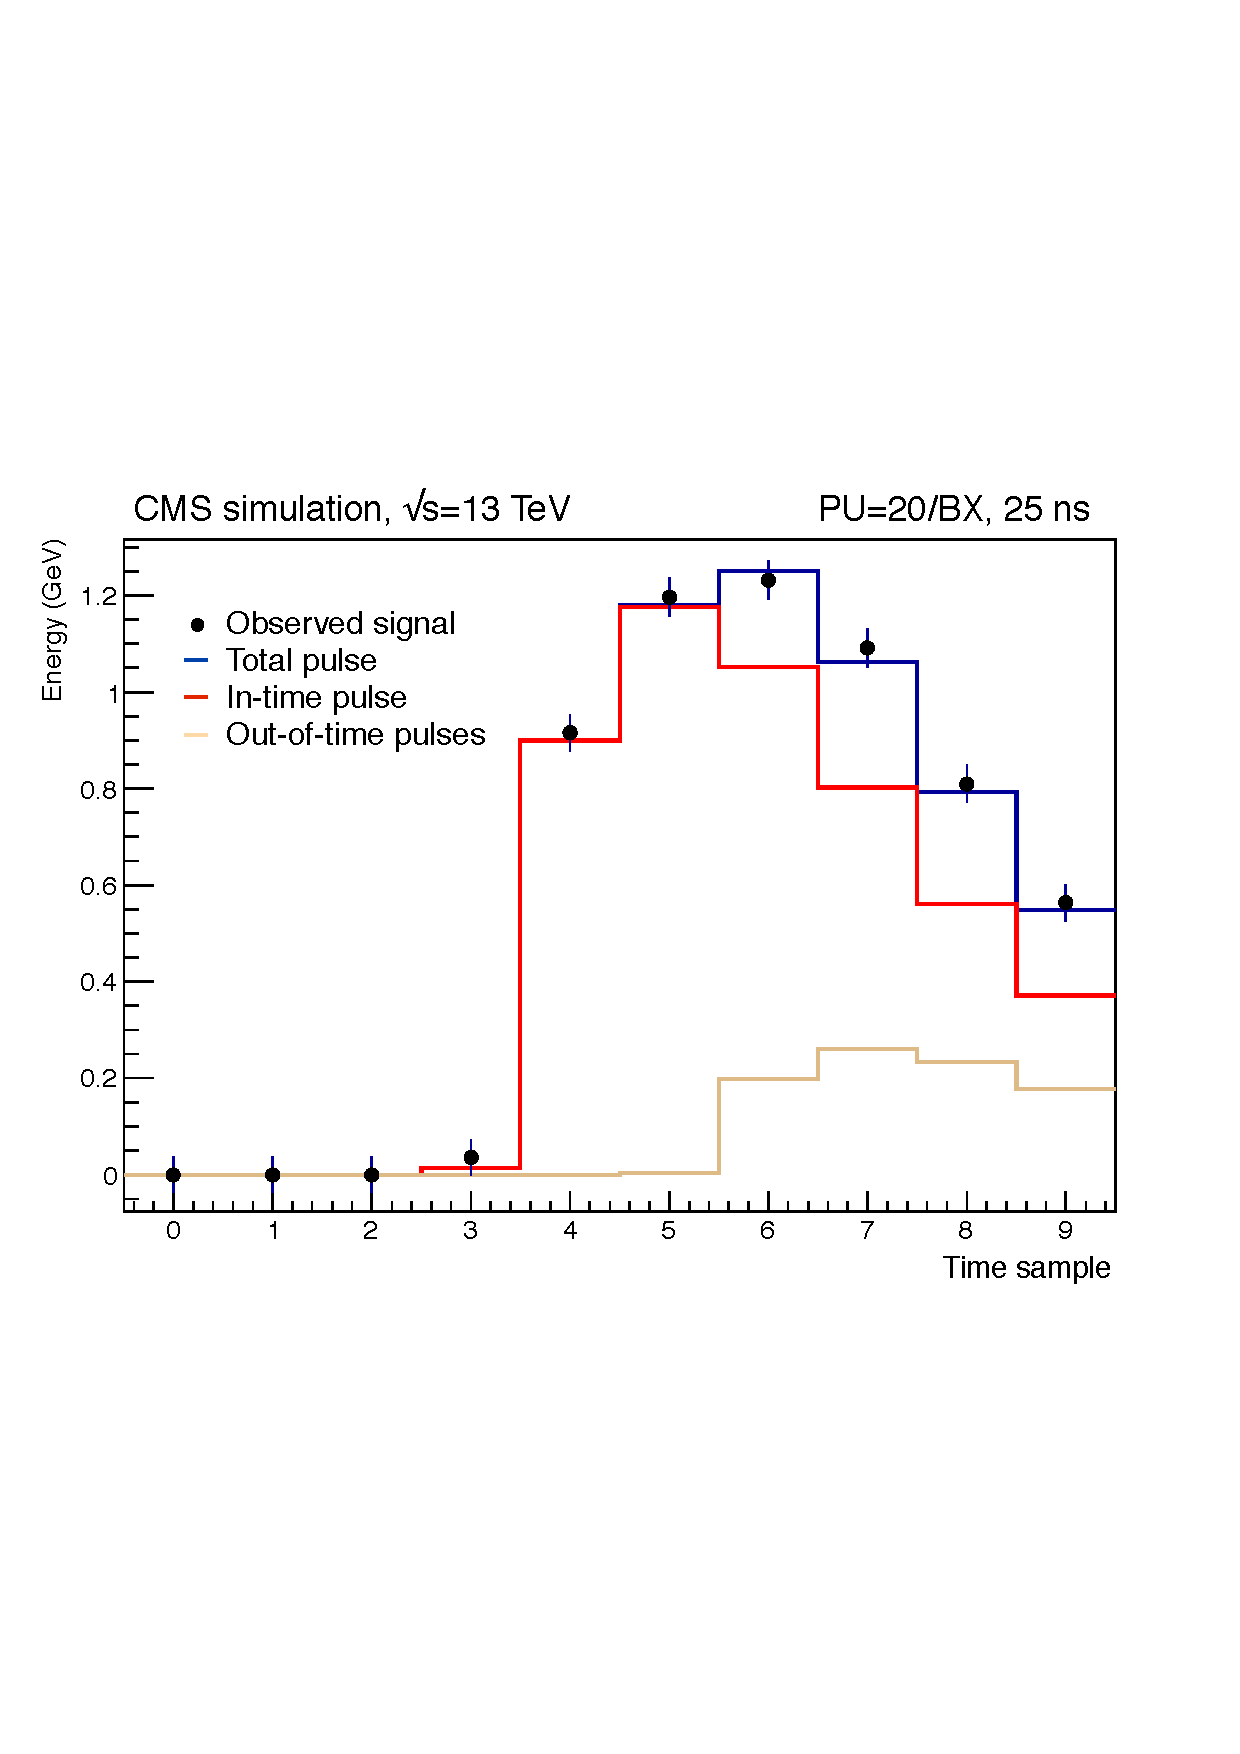
\includegraphics[width=0.5\textwidth]{plot/multifit_EB.pdf}
	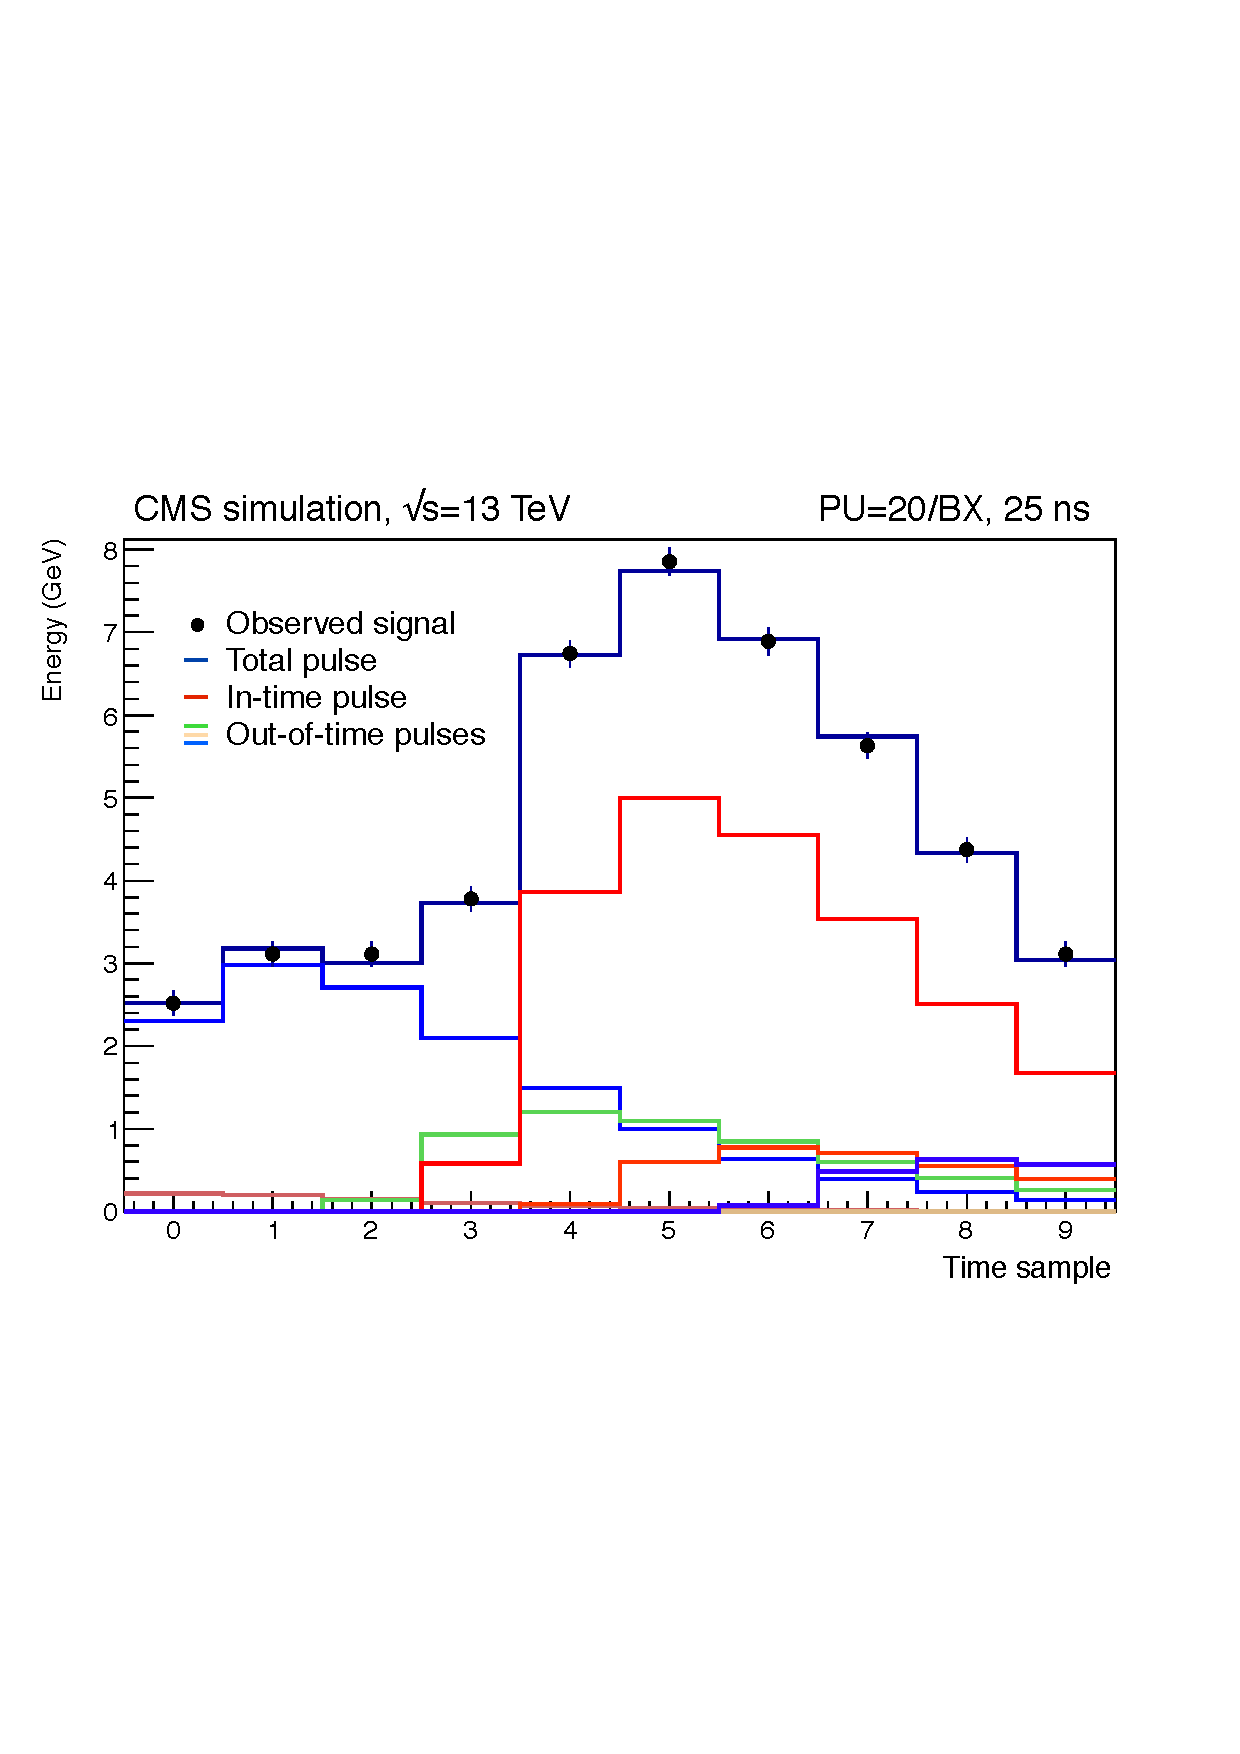
\includegraphics[width=0.5\textwidth]{plot/multifit_EE.pdf}
	\caption{Examples of fitted pulses for signals in the EB (left) and in the EE (right) with 20 pileup interactions.}
	\label{fig:multifit}
\end{figure*}

Energy of the photons usually spread over several crystals. 
Calorimeter hits deposited by the same electromagnetic shower is collected by the clustering algorithm. 
First, cluster seeds are formed by taking local maxima of energy deposits above a given threshold. 
Second, adjacent cells with an energy above the noise cut are added to the cluster seeds to form basic clusters. 
In the final step, basic clusters belonging to the same object are merged together to form a supercluster, which is extended in $\phi$, to recover the radiated energy. 
The shower energy can be estimated as:
\begin{equation}
      E_{e, \gamma} = F_{e, \gamma} \cdot [ G \cdot  \displaystyle\sum_{i} S_i(t) \cdot C_i \cdot A_i + E_{ES}],
\end{equation}
where the sum runs over all clustered crystals. The quantity $A_i$ is the pulse
amplitude, which is converted to a GeV scale by multiplying the calibration
factor $G$, and $S_i(t)$ is a correction term that accounts for the time
variations of the channel response with $C_i$ being the inter-calibration
factor. For showers in the EE the energy measured by the preshower
($E_{ES}$) is added. Finally, the energy correction term $F_{e, \gamma}$
is applied to take into account geometry and upstream material
effects, as well as the difference between electron and photon showers. 

In-situ ECAL calibrations with physics events are applied to the EM clusters to improve the energy resolution. 
There are two steps of calibrations, inter-calibration and energy scale calibration, applied on top of the responses corrections of single ECAL channels. 
The purpose of inter-calibration is to equalize the variations in channel response due to different crystal light-yield and photo-detector gains. 
The inter-calibration factors are measured using multiple methods, including the use of the azimuthal symmetry of energy deposit in minimum bias events, the diphoton invariant mass of $\pi^0$ and $\eta^0$ decays, the E/p ratio of electrons from W and Z decays, and the mass peak of $\mathrm{Z}\rightarrow e^+e^-$ decays. 
The combined coefficient is obtained by taking the mean value of individual corrections weighted by their respective precisions. 
The energy scale calibration, on the other hand, is applied to convert the digitized signal to GeV. 
The absolute ADC to GeV scale factor is determined separately in EB and EE using the $\mathrm{Z}\rightarrow e^+e^-$ invariant mass peak, matching the reconstructed mass in data to that in simulation. 

Any object that deposits a significant fraction of energy in the ECAL can be reconstructed as a photon.
Therefore, electrons and electromagnetically rich jets are all registered in the photon collection. 
To distinguish the real photons from other objects, photon candidates are required to pass a list of shower shape quality cuts and not to have a matching track seed from the tracker. 
Details of photon identification criteria is described in Section \ref{sed:photonID}.

\section{Electrons}

Electrons are reconstructed by associating a track reconstructed in the silicon tracker to an ECAL supercluster~\cite{ElectronPF}.
A dedicated track reconstruction algorithm is implemented for electrons because they have large radiative losses in the tracker than other charged particles.
The electron track reconstruction also has the seeding, track finding and track fitting steps. 
In the seeding step, both ECAL-based and tracker-based seeding are considered. 
The track building starts with track reconstructions using the KF algorithm, with the track hits collected up to the ECAL. 
This method works well for electrons with negligible radiative loss. 
In the case of large bremsstrahlung, the KF reconstruction will fail and a dedicated Gaussian sum filter (GSF) is applied. 
The GSF models the energy loss in each tracker layer by a mixture of Gaussian distributions.
The use of GSF improves the momentum resolution of electrons. 

An electron is identified when the GSF track can be associated with an ECAL cluster. 
For the ECAL-seeded electrons, the SCs are propagated inwards to the inner tracker layers under the assumption that the energy-weighted positions of the clusters are on the trajectory of the electrons. 
The ECAL-predicted hits are then matched geometrically to the GSF tracks with the following requirements: 
\begin{itemize}
	\item $|\Delta\eta| < $ 0.02, with $|\Delta\eta|$ being the distance in $\eta$ between the SC and track $\eta$ extrapolated to the position of closest approach to the SC
	\item $|\Delta\phi| < $ 0.15, with  $|\Delta\phi|$ being the distance in $\phi$
\end{itemize}
For tracker-seeded electrons, the matching between the tracks and clusters are evaluated by the Multivariate Analysis (MVA) technique. 

The overall reconstruction efficiency is $\sim$ 93\% for electrons from Z decay.
For collision data, the efficiency is measured to be 88-98\% in the barrel and 90-96\% in the endcaps in the $p_T$ range from 10 to 100 GeV.

\section{Jets}
Jet is a collimated spray of hadrons as a result of the hadronisation of quarks or gluons. 
Depending on the fraction of final particles produced by hadronization, a jet may contain hadrons, non-isolated electrons and collinear photons. 
Thus multiple sub-detectors can have energy deposits from a jet.
A combination of these signals is performed with jet algorithms~\cite{FastJet} to form a reconstructed jet. 

The jets used in this analysis are reconstructed with the anti-$k_T$ algorithms~\cite{AntiKT}. 
In this algorithm, each entity $i$ (particles, pseudojets) is assigned a distance to the beam (B): 
\begin{equation}
	d_{iB} = k_{ti}^{2p},
\end{equation}
where $k_{ti}$ is the transverse momentum of particle $i$. Here we use $p = -1$, and this is why this algorithm is named as ``anti-$k_T$''. 
The distance between two entities is defined as:
\begin{equation}
	d_{ij} = min(k_{ti}^{2p}, k_{tj}^{2p})\frac{\Delta_{ij}^2}{R^2},
\end{equation}
where $\Delta_{ij}^2 = (\eta_i - \eta_j)^2 + (\phi_i - \phi_j)^2$ and R is the radius of the reconstruction cone. 
In CMS Run II, a R = 0.4 cone is used for normal jets. 

The anti-$k_T$ is a sequential clustering algorithm which proceeds in an iterative way.
In each iteration, it computes the $d_{iB}$ and $d_{ij}$ of all entities, and compares them to find the smallest quantity.  
If $d_{ij}$ is the smallest one, then the $i$th and $j$th object are merged into one. 
Otherwise, if $d_{iB}$ is the smallest one, then the $i$th object is called a jet and get removed from the list. 
These steps are repeated until all particles are clustered into jets. 

\section{Muons}
Muons leave hits in both the inner tracker and muon stations.
The tracker can measure the momentum of muons with high precision, while the muon stations can detect the muons with higher purity because other particles are absorbed in the calorimeter system. 
Muons can be reconstructed in an inside-out, outside-in or standalone way in CMS~\cite{MuonPF}.
Based on the reconstruction method, the muons can be classified into three types: 
\begin{itemize}
	\item Standalone Muon. Hits in the muon chambers are grouped to form standalone tracks, which provides an initial estimate of the muon tracks and can be used as seeds.
	\item Global Muon. A track reconstructed in the inner tracker is assigned to a standalone muon if they propagate to the same position onto a common surface. 
	\item Tracker Muon. All reconstructed tracks are considered as muons and are extrapolated to the muon chambers. If the track can match at least one muon segment, it is recognized as a tracker muon. 
\end{itemize}
These types are not mutually exclusive.
The muon identification criteria usually require the muon to be two or more of these types. 

\section{Missing Transverse Momentum}
Particles that do not interact with the detector materials, such as neutrinos, usually escape the detector, carrying part of the energy of the final states.
In the initial state, the total momentum in the transverse plane is almost zero. 
The presence of invisible particles, therefore, results in an imbalance in the transverse plane, which is named as missing transverse momentum, denoted as \MET.

The raw \MET~is calculated as the negative of the vector sum of the transverse momentum of all reconstructed objects in an event~\cite{METPF}:
\begin{equation*}
	p_{T, raw}^{miss} = - \sum_{i}^{N_{particles}}p_{T,i}
\end{equation*}

\MET~is a high-level variable reconstructed using all visible particles in an event.
It is sensitive to anomalous signals in the detector.
Such anomalous signals include unphysical energy deposits in the calorimeter, noise of detector, beam-induced backgrounds, and poorly instrumented regions of the detector.
Dedicated event filters are designed to identify and remove these anomalies. 

\end{document}


